\documentclass[12pt]{book}
\usepackage{booktabs}
\usepackage[table]{xcolor}
\usepackage{tcolorbox}
\usepackage[T1]{fontenc}
\usepackage{wrapfig}
\usepackage{url}
\usepackage{dsfont}
\usepackage{enumitem}
\usepackage{array}
\usepackage{booktabs}

\usepackage{mathtools, nccmath}
\usepackage[polish]{babel}
\usepackage[utf8]{inputenc}
\usepackage{lmodern}
\usepackage{pifont}
\usepackage{blkarray, bigstrut}
\usepackage{amsmath}
\usepackage{kbordermatrix}
\usepackage{cases}
\usepackage{graphicx}
\usepackage{cellspace}
\usepackage[T1]{fontenc}
\usepackage{amsthm}
\selectlanguage{polish}
\usepackage{amsmath}
\usepackage{graphicx}
\usepackage{float}
\usepackage{cite}
\usepackage[margin=2.5cm]{geometry}
\theoremstyle{plain}
\newtheorem{definicja}{Definicja}
\newtheorem{twr}{Twierdzenie}
\newtheorem{lem}[twr]{Lemat}
\newtheorem{mur}{Murphy}[section]
\newcolumntype{P}[1]{>{\centering\arraybackslash}p{#1}}
\newcommand\green{\cellcolor{green!10}}
\newcommand\cincludegraphics[2][]{\raisebox{-0.5\height}{\includegraphics[#1]{#2}}}
\newcommand\red{\cellcolor{red!20}}
\newcommand\blue{\cellcolor{blue!20}}
\newcommand{\R}{\mathbb{R}}
\newcommand*{\tabbox}[2][t]{%
	\vspace{0pt}\parbox[#1][3.7\baselineskip]{1cm}{\strut#2\strut}}
\newcommand\addtag{\refstepcounter{equation}
	\renewcommand{\labelenumii}{\theenumii}
	\renewcommand{\theenumii}{\theenumi.\arabic{enumii}.}
	\tag{\theequation}}

\begin{document}
	\title{Optymalizacja  systemu sygnalizacji świetlnej w 
		oparciu o przepływowy model ruchu pojazdów.}
	\author{Michał Lis}
	\date{\today}
	\maketitle
	\tableofcontents
	
	\chapter {Środowiska symulacyjne i ich nauka}
	\section{Środowisko 1}
	\begin{figure}[H]
		\centering
		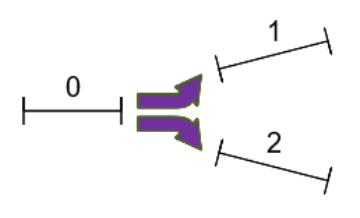
\includegraphics[width=7cm]{images/env_1}
		\label{fig:env_1}
		\caption{Środowisko 1}
	\end{figure}
	
	Środowisko posiada 3 jednokierunkowe drogi. Każda droga ma 1 odcinek co daje w sumie 3 odcinki (są numerowane od 0 co widać na rysunku \ref{fig:env_1}).
	W sieci dróg znajduje się 1 skrzyżowanie. Jest do niego przypisany agent, który odpowiada za sterowanie sygnalizacją świetlną. 
	
	\subsection{Fazy świetlne}
	Skrzyżowanie posiada 3 fazy świetlne. Faza 0 i 1 umożliwiają skręt odpowiednio w lewo i w prawo. Automatycznie ustawiana jest faza żółtych świateł przez 2 interwały czasowe w przypadku podjęcia akcji zmiany faz z 0 na 1 lub odwrotnie. 
	
	\begin{figure}[H]
		\centering
		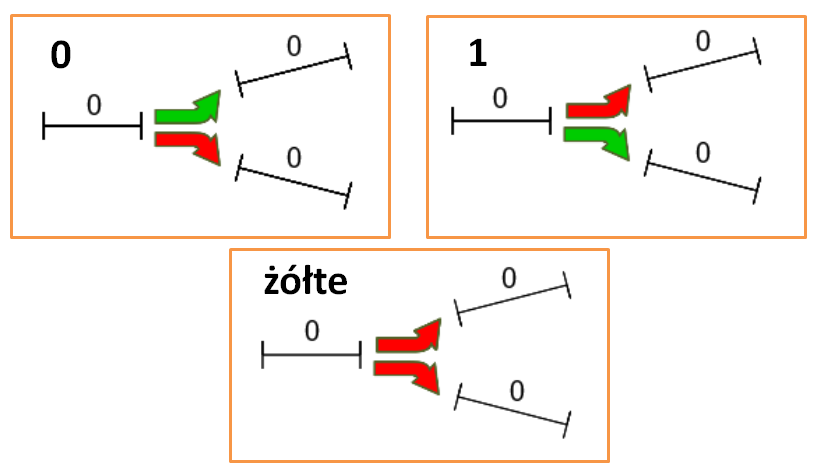
\includegraphics[width=14cm]{images/env_1_fazy}
		\label{fig:env_1_fazy}
		\caption{Środowisko 1 - fazy świateł}
	\end{figure}
	
	\subsection{Przepływ pojazdów}
	30 procent pojazdów będących na odcinku 0 ma zamiar jazdy w lewo. Pozostałe 70 procent skręca w prawo. 
	\begin{figure}[H]
		\centering
		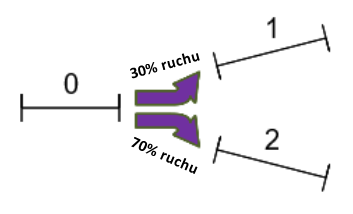
\includegraphics[width=14cm]{images/env_1_ruch}
		\label{fig:env_1_ruch}
		\caption{Środowisko 1 - prawdopodobienstwa przejazdów}
	\end{figure}
	
	Definiuje to następującą macierz prawdopodobienstwa przejazdow:
	\def \P {\begin{bmatrix}
			0 & 0 & 0 \\
			0.3 & 0 & 0 \\
			0.7 & 0 & 0 \\
	\end{bmatrix}}
	
	\[
	P=\P \addtag
	\]
	
	
	\subsection{Macierze świateł i stanowe dla poszczególnych faz świateł}
	
	
	\def \Azero {\begin{bmatrix}
			0.7 & 0 & 0 \\
			0.3 & 0 & 0 \\
			0   & 0 & 0 \\
	\end{bmatrix}}
	\def \AI {\begin{bmatrix}
			0.3 & 0 & 0 \\
			0   & 0 & 0 \\
			0.7 & 0 & 0 \\
	\end{bmatrix}}
	\def \Azolte {\begin{bmatrix}
			1 & 0 & 0 \\
			0 & 0 & 0 \\
			0 & 0 & 0 \\
	\end{bmatrix}}
	\def \Szero {\begin{bmatrix}
			0 & 0 & 0 \\
			1 & 0 & 0 \\
			0   & 0 & 0 \\
	\end{bmatrix}}
	\def \SI {\begin{bmatrix}
			0 & 0 & 0 \\
			0   & 0 & 0 \\
			1 & 0 & 0 \\
	\end{bmatrix}}
	\def \Szolte {\begin{bmatrix}
			0 & 0 & 0 \\
			0 & 0 & 0 \\
			0 & 0 & 0 \\
	\end{bmatrix}}
	
	Macierze swiatel $S$ oraz stanowe $A$ sa nastepujace w zaleznosci od fazy.
	\newline
	\begin{table}
		\centering
		\begin{tabular}{| Sc | c | c |}
			\hline
			\textbf{Faza} & $\textbf{S}$ & $\textbf{A}$ \\
			\hline
			\cincludegraphics[height=3cm]{images/env_1_faza_0} & $\Szero$  & $\Azero$ \\
			\hline 
			\cincludegraphics[height=3cm]{images/env_1_faza_1} & $\SI$  & $\AI$ \\
			\hline
			\cincludegraphics[height=3cm]{images/env_1_faza_zolte} & $\Szolte$  & $\Azolte$ \\
			\hline
		\end{tabular}
	\end{table}
	
	
	\subsection{Korki}
	Powyższe przedstawienie macierzy stanowej nie zawiera w sobie jeszcze pojęcia korka. W jednym interwale czasowym może przejechać przez skrzyżowanie astronomiczna wręcz liczba pojazdów. Dodane zostanie zatem ograniczenie do maksymalnie 10 pojazdów przejeżdżających w trakcie jednego interwału czasowego.
	Należy sformułować funkcję, która określi przepływ z uwzględnieniem tworzenia się korka w przypadku większej liczby pojazdów.
	Niech $i,j$ oznaczają rozważane odcinki wlotowe i wylotowe. Wtedy funkcja korka jest następująca:
	\begin{numcases}{f(i,j)=}
	0 & dla $S[i,j]=0$ - czerwone światło \\
	P[i,j] & dla $ S[i,j]=1 \wedge P[i,j] x[i]<10$ - zielone światło, bez korka \\
	\frac{10}{x[i]} & dla $S[i,j]=1  \wedge P[i,j] x[i] \geq 10$ - zielone światło i korek
	\end{numcases}
	Wtedy macierz stanowa $A$ przedstawia się następująco:
	
	\def \A_f {\begin{bmatrix}
			1-f(0,1)-f(0,2) & 0 & 0 \\
			f(0,1) & 0 & 0 \\
			f(0,2)   & 0 & 0 \\
	\end{bmatrix}}
	
	
	\[A=\A_f \]
	
	Warto zauważyć, że chociaż mamy teraz jeden wzór na macierz stanową, to dalej A jest zależne nie tylko od fazy świateł, ale także ilości pojazdów na poszczególnych odcinkach (w przypadku tego Środowiska jedynie od ilości pojazdów na odcinku 0).
	
	\subsection{Końcowe równanie stanu - podsumowanie wzorów matematycznych}
	
	Równanie stanu jest następujące:
	\[
	x(t)=A(t-1)x(t-1)+u(t-1)
	\]
	Równanie macierzy stanowej to:
	\[A=\A_f \]
	Funkcja f jest zdefiniowana następująco:
	\begin{numcases}{f(i,j)=}
	0 & dla $S[i,j]=0$ - czerwone światło \\
	P[i,j] & dla $ S[i,j]=1 \wedge P[i,j] x[i]<10$ - zielone światło, bez korka \\
	\frac{10}{x[i]} & dla $S[i,j]=1  \wedge P[i,j] x[i] \geq 10$ - zielone światło i korek
	\end{numcases}
	Macierzą prawdopodobieństwa jest:
	\[
	P=\P \addtag
	\]
	Macierze sygnalizacji świetlnej S są następujące dla poszczególnych faz:
	\newline
	\begin{table}
		\centering
		\begin{tabular}{| Sc | c |}
			\hline
			\textbf{Faza} & $\textbf{S}$  \\
			\hline
			\cincludegraphics[height=3cm]{images/env_1_faza_0} & $\Szero$   \\
			\hline 
			\cincludegraphics[height=3cm]{images/env_1_faza_1} & $\SI$  \\
			\hline
			\cincludegraphics[height=3cm]{images/env_1_faza_zolte} & $\Szolte$ \\
			\hline
		\end{tabular}
	\end{table}
	\newline
	Ciąg wektorów $u$ określa pojazdy napływające do układu. Pierwszy element trójelementowy wektora $u(t-1)$ jest dowolny i określa ilość pojazdów, które wjeżdżają na odcinek 0. Pozostałe 2 elementy wektora $u(t-1)$ to zera, bo tylko na początku odcinka 0 istnieje źródło ruchu.
	
\end{document} 













